\chapter{Noise, Variance and Experiments}\label{chap:noise}

\Cref{chap:smm} showed that in the noiseless setting the parity schedule of
Switching MM\index{Switching MM} is not an acceleration device. On a quadratic, \smmdet\ is a
period two step size schedule with steps $\alpha$ and $(1+\beta)\alpha$
(\cref{thm:smmquad}); in the slow directions it improves the constant of
gradient descent by the factor $m_{\mathrm{SMM}}=(2+\beta)/2$ and is beaten by
every step momentum\index{momentum}, whose factor is $1/(1-\beta)$. If SMM has a reason to
exist, that reason must lie elsewhere.
A natural hope is that the parity schedule acts as a \emph{variance filter}: momentum recycles gradient shocks through its memory, and a method that uses its memory only half the time ought to recycle less noise.

This chapter puts that hope to an exact test. After recalling the classical
AR(2) analysis of every step momentum under additive gradient noise, we prove
the corresponding exact result for \smmdet, \cref{thm:smmvar}. In the slow
modes SMM amplifies noise, relative to gradient descent at the same step, by
$(2+2\beta+\beta^2)/(2+\beta)$: this is $1.359$ at the Collatz value of
$\beta$ and never exceeds $5/3$, whereas every step momentum amplifies by the
unbounded factor $1/(1-\beta)$.
Compared at matched speed in the slow modes rather than at matched step, SMM has no advantage over gradient descent in those modes, although it is quieter in the fast ones; it is quieter than every step momentum largely because it moves more cautiously.
Its genuine
virtue is robustness: its noise behaviour hardly depends on $\beta$, which is
the precise content of the claim that SMM is a low tuning method.
The second half of the chapter presents experiments with SMM, rerun for this book, and reconciles them quantitatively with the theory.

\section{A model of gradient noise}\label{sec:ch7:model}

We work with the strongly convex quadratic
$f(x)=\tfrac12x^\top Ax-b^\top x$, $A$ symmetric positive definite with
eigenvalues in $[\mu,L]$, and suppose that the algorithm does not see
$\nabla f$ but a noisy version
\begin{equation}\label{eq:ch7:oracle}
  g(x)=\nabla f(x)+\xi,
\end{equation}
where a fresh $\xi$ is drawn at every call, independent of the past, with mean
zero and covariance $\sigma^2I$. This is the simplest model of a stochastic
gradient; it ignores the state dependence and anisotropy of minibatch noise,
but isolates how a method turns independent shocks into fluctuations of the
iterate. Every method we consider decouples along the eigenvectors of $A$. Fix
an eigenvalue $\lambda$, write $a=\alpha\lambda$ for the normalized step,
$e_t$ for the component of $x_t-x^\ast$ and $\xi_t$ for the component of the
noise drawn at iteration $t$; the $\xi_t$ are independent with mean zero and
variance $\sigma^2$. With $\alpha=1/L$, $a$ ranges over $[1/\kappa,1]$. Each
scalar error has a variance that converges to a limit, the \emph{stationary
variance}, and since
\begin{equation}\label{eq:ch7:gap}
  \E\bigl[f(x_t)-f(x^\ast)\bigr]=\tfrac12\sum_{\lambda}\lambda\,\E[e_t(\lambda)^2],
\end{equation}
these limits determine the noise floor\index{noise floor} that remains after the
deterministic transient has died away.

For gradient descent, $e_{t+1}=(1-a)e_t-\alpha\xi_t$, an autoregression of
order one, and the stationary variance is
\begin{equation}\label{eq:ch7:gd}
  V_{\mathrm{GD}}(a)=\frac{\alpha^2\sigma^2}{1-(1-a)^2}
  =\frac{\alpha^2\sigma^2}{a(2-a)},\qquad 0<a<2.
\end{equation}
In the slow modes $V_{\mathrm{GD}}\approx\alpha^2\sigma^2/(2a)=\alpha\sigma^2/(2\lambda)$:
the floor is proportional to the step. A longer step is faster and noisier in
exactly compensating amounts, and every comparison below must account for
this.

\section{Every step momentum as an autoregression}\label{sec:ch7:ar2}

\subsection{The stationary variance of an AR(2) process}

The classical tool is an elementary lemma on autoregressions of order two;
see Brockwell\index{Brockwell, P. J.} and Davis\index{Davis, R. A.}~\cite{brockwell1991} for the general theory.

\begin{lemma}[Stationary variance of an AR(2) process]\label{lem:ch7:ar2}
Let $e_{t+1}=a_1e_t+a_2e_{t-1}+\varepsilon_t$ with $\varepsilon_t$ independent,
mean zero, variance $s^2$, and $\varepsilon_t$ independent of
$(e_t,e_{t-1})$. Suppose both roots of $z^2-a_1z-a_2$ lie in the open unit
disc, which holds if and only if
\begin{equation}\label{eq:ch7:triangle}
  |a_2|<1,\qquad 1-a_1-a_2>0,\qquad 1+a_1-a_2>0 .
\end{equation}
Then $\Var(e_t)$ converges, from any initial condition with finite second
moments, to
\begin{equation}\label{eq:ch7:ar2var}
  \gamma_0=\frac{(1-a_2)\,s^2}{(1+a_2)\bigl((1-a_2)^2-a_1^2\bigr)} .
\end{equation}
\end{lemma}

\begin{proof}
In state form the covariance of $(e_t,e_{t-1})$ obeys an affine recursion
whose linear part has spectral radius equal to the square of that of the
companion matrix, which is less than one; so it converges geometrically to its
unique fixed point. In stationarity let $\gamma_k=\Cov(e_t,e_{t-k})$.
Multiplying the recursion by $e_t$, by $e_{t-1}$ and by $e_{t+1}$ and taking expectations
gives the Yule and Walker equations
\[
  \gamma_1=a_1\gamma_0+a_2\gamma_1,\qquad
  \gamma_2=a_1\gamma_1+a_2\gamma_0,\qquad
  \gamma_0=a_1\gamma_1+a_2\gamma_2+s^2 .
\]
The first gives $\gamma_1=a_1\gamma_0/(1-a_2)$. Substituting the second into
the third, $\gamma_0(1-a_2^2)=a_1(1+a_2)\gamma_1+s^2
=a_1^2(1+a_2)\gamma_0/(1-a_2)+s^2$. Multiplying by $1-a_2$ and collecting terms
gives $\gamma_0(1+a_2)\bigl((1-a_2)^2-a_1^2\bigr)=(1-a_2)s^2$, which is
\eqref{eq:ch7:ar2var}. The conditions \eqref{eq:ch7:triangle} are the classical
stability triangle for a real quadratic.
\end{proof}

\subsection{Heavy ball}

The noisy heavy ball\index{heavy ball} iteration
$x_{t+1}=x_t-\alpha g(x_t)+\beta(x_t-x_{t-1})$ gives, on an eigendirection,
\begin{equation}\label{eq:ch7:hbrec}
  e_{t+1}=(1+\beta-a)\,e_t-\beta\,e_{t-1}-\alpha\xi_t,
\end{equation}
an AR(2) process with $a_1=1+\beta-a$, $a_2=-\beta$ and $s^2=\alpha^2\sigma^2$.

\begin{proposition}[Heavy ball under additive noise]\label{prop:ch7:hb}
Let $0\le\beta<1$ and $0<a<2(1+\beta)$. The stationary variance of
\eqref{eq:ch7:hbrec} is
\begin{equation}\label{eq:ch7:hbvar}
  V_{\mathrm{HB}}(a)=\frac{\alpha^2\sigma^2\,(1+\beta)}{(1-\beta)\,a\,\bigl(2(1+\beta)-a\bigr)} .
\end{equation}
As $a\to0$, $V_{\mathrm{HB}}(a)\sim\alpha^2\sigma^2/\bigl(2a(1-\beta)\bigr)$, so
$V_{\mathrm{HB}}/V_{\mathrm{GD}}\to1/(1-\beta)$.
\end{proposition}

\begin{proof}
The conditions \eqref{eq:ch7:triangle} read $\beta<1$, $1-a_1-a_2=a>0$ and
$1+a_1-a_2=2(1+\beta)-a>0$, which are the hypotheses. In
\eqref{eq:ch7:ar2var}, $1-a_2=1+\beta$, $1+a_2=1-\beta$, and
\[
  (1-a_2)^2-a_1^2=(1+\beta)^2-(1+\beta-a)^2=a\bigl(2(1+\beta)-a\bigr).
\]
This is \eqref{eq:ch7:hbvar}. For small $a$ the last factor is
$2(1+\beta)+O(a)$, the factors $1+\beta$ cancel, and the limit follows on
dividing by $V_{\mathrm{GD}}\sim\alpha^2\sigma^2/(2a)$.
\end{proof}

The factor $1/(1-\beta)$ is $2.409$ at $\beta=\lt-1$, $3$ at $\beta=2/3$ and $10$
at $\beta=0.9$. Its origin is easy to see. In the slow regime the characteristic
polynomial has a fast root near $\beta$ and a slow root $1-a/(1-\beta)+O(a^2)$.
A shock $\alpha\xi_t$ enters the velocity, and by the time the fast root has
dissipated it the position has moved by
$\alpha\xi_t(1+\beta+\beta^2+\cdots)=\alpha\xi_t/(1-\beta)$. Momentum thus
multiplies the effective step by $m=1/(1-\beta)$, speeding the slow mode up by
$m$, and multiplies each shock by $m$, hence its variance by $m^2$; the net
effect on the floor is $m^2/m=m$. We return to this bookkeeping in
\cref{sec:ch7:efficiency}.

\subsection{Nesterov}

Constant momentum\index{momentum} Nesterov\index{Nesterov acceleration} evaluates the noisy gradient at the extrapolated
point: $y_t=x_t+\beta(x_t-x_{t-1})$, $x_{t+1}=y_t-\alpha g(y_t)$. On an
eigendirection,
\begin{equation}\label{eq:ch7:nagrec}
  e_{t+1}=(1-a)(1+\beta)\,e_t-(1-a)\beta\,e_{t-1}-\alpha\xi_t .
\end{equation}

\begin{proposition}[Nesterov under additive noise]\label{prop:ch7:nag}
Let $0\le\beta<1$ and $0<a\le1$. The stationary variance of
\eqref{eq:ch7:nagrec} is
\begin{equation}\label{eq:ch7:nagvar}
  V_{\mathrm{NAG}}(a)=\frac{\alpha^2\sigma^2\,(1+\beta-a\beta)}
  {a\,(1-\beta+a\beta)\,\bigl(2(1+\beta)-a(1+2\beta)\bigr)} .
\end{equation}
As $a\to0$, $V_{\mathrm{NAG}}/V_{\mathrm{GD}}\to1/(1-\beta)$, the same slow mode
amplification as heavy ball\index{heavy ball}; at $a=1$, $V_{\mathrm{NAG}}=V_{\mathrm{GD}}=\alpha^2\sigma^2$.
\end{proposition}

\begin{proof}
Here $a_1=(1-a)(1+\beta)$ and $a_2=-(1-a)\beta$, so $|a_2|<1$,
$1-a_1-a_2=1-(1-a)=a>0$ and $1+a_1-a_2=1+(1-a)(1+2\beta)>0$; the lemma applies.
Now $1-a_2=1+\beta-a\beta$, $1+a_2=1-\beta+a\beta$, and
\[
  (1-a_2)^2-a_1^2=(1-a_2-a_1)(1-a_2+a_1)=a\bigl(2(1+\beta)-a(1+2\beta)\bigr)
\]
since $1-a_2+a_1=1+\beta-a\beta+(1-a)(1+\beta)=2(1+\beta)-a(1+2\beta)$.
Substituting in \eqref{eq:ch7:ar2var} gives \eqref{eq:ch7:nagvar}, and both
limits are immediate.
\end{proof}

Heavy ball and Nesterov agree in the slow modes and differ for larger $a$: at
$a=1$ the Nesterov error is just the last shock, while heavy ball still carries
momentum.

\section{The exact variance of Switching MM}\label{sec:ch7:smmvar}

For \smmdet\ the coefficients alternate with the parity of $t$, so the error is
not a stationary AR(2) process. The way through is \cref{lem:ch6:ystep}, which
holds for any gradient oracle and therefore for the noisy one: starting from an
even index, the extrapolated point is a single long step from $x_t$ using the
\emph{same} noisy gradient,
\[
  y_{t+1}=x_{t+1}+\beta(x_{t+1}-x_t)=x_t-(1+\beta)\alpha\,g(x_t).
\]
The noise drawn at the even step is therefore used twice, once in the descent
step and once more, scaled by $\beta$, through the extrapolation. Two steps of
SMM consume two independent shocks with weights $(1+\beta)\alpha$ and $\alpha$,
exactly as noisy gradient descent with the cyclic step\index{cyclic step sizes}s $(1+\beta)\alpha$ and
$\alpha$ would.

\begin{theorem}[Stationary variance of \smmdet]\label{thm:smmvar}
Let $f$ be the quadratic of \cref{sec:ch7:model}, with the noisy oracle
\eqref{eq:ch7:oracle}, let $0\le\beta<1$, and fix an eigendirection with
$a=\alpha\lambda\in(0,1]$. Let
\[
  \rho=(1-a)\bigl(1-(1+\beta)a\bigr).
\]
\begin{enumerate}[label=(\roman*),leftmargin=2em]
\item For every even $t$ the error of \smmdet\ satisfies the exact two step
recursion
\begin{equation}\label{eq:ch7:twostep}
  e_{t+2}=\rho\,e_t+w_t,\qquad
  w_t=-(1-a)(1+\beta)\alpha\,\xi_t-\alpha\,\xi_{t+1},
\end{equation}
where the $w_t$, $t$ even, are independent, independent of $e_t$, with mean zero and
$\Var(w_t)=\alpha^2\sigma^2\bigl[(1-a)^2(1+\beta)^2+1\bigr]$.
\item As $t\to\infty$ through even values, $\Var(e_t)$ converges to
\begin{equation}\label{eq:ch7:veven}
  V_{\mathrm{even}}=\frac{\alpha^2\sigma^2\bigl[(1-a)^2(1+\beta)^2+1\bigr]}{1-\rho^2},
\end{equation}
and through odd values to
\begin{equation}\label{eq:ch7:vodd}
  V_{\mathrm{odd}}=(1-a)^2\,V_{\mathrm{even}}+\alpha^2\sigma^2 .
\end{equation}
\item The phase averaged stationary variance
$V_{\mathrm{SMM}}=\tfrac12(V_{\mathrm{even}}+V_{\mathrm{odd}})$ is the rational
function
\begin{equation}\label{eq:ch7:vavg}
  \frac{V_{\mathrm{SMM}}(a)}{\alpha^2\sigma^2}
  =\frac{Q(a,\beta)}{1-\rho^2},
\end{equation}
with
\begin{align*}
  Q(a,\beta)&=(2+2\beta+\beta^2)-(1+\beta)(2+3\beta)\,a\\
  &\quad+(1+\beta)(1+3\beta)\,a^2-\beta(1+\beta)\,a^3,\\
  1-\rho^2&=a\bigl(2+\beta-(1+\beta)a\bigr)\bigl(2-(2+\beta)a+(1+\beta)a^2\bigr).
\end{align*}
\end{enumerate}
\end{theorem}

\begin{proof}
(i) Let $t$ be even. The descent step gives
$e_{t+1}=(1-a)e_t-\alpha\xi_t$, so $e_{t+1}-e_t=-ae_t-\alpha\xi_t$ and the
extrapolated point has error
\[
  e_{t+1}+\beta(e_{t+1}-e_t)
  =\bigl(1-(1+\beta)a\bigr)e_t-(1+\beta)\alpha\xi_t .
\]
The injection step evaluates a noisy gradient at this point, with fresh noise
$\xi_{t+1}$, and multiplies the error by $1-a$:
\[
  e_{t+2}=(1-a)\bigl[\bigl(1-(1+\beta)a\bigr)e_t-(1+\beta)\alpha\xi_t\bigr]-\alpha\xi_{t+1},
\]
which is \eqref{eq:ch7:twostep}. The error $e_t$ is a function of $e_0$ and of
$\xi_0,\dots,\xi_{t-1}$, while $w_t$ is a function of $\xi_t$ and $\xi_{t+1}$;
for distinct even $t$ the pairs $(\xi_t,\xi_{t+1})$ are disjoint. This gives the
independence claims, and the variance of $w_t$ is the sum of the variances of its
two independent terms.

(ii) By (i), $\Var(e_{t+2})=\rho^2\Var(e_t)+\Var(w_t)$ for even $t$. By
\cref{cor:ch6:stability}, $|\rho|<1$ whenever $0<a<(2+\beta)/(1+\beta)$, in
particular for $a\in(0,1]$, so this affine recursion converges geometrically to
its fixed point \eqref{eq:ch7:veven}. For odd times, $e_{t+1}=(1-a)e_t-\alpha\xi_t$
with $\xi_t$ independent of $e_t$, so $\Var(e_{t+1})=(1-a)^2\Var(e_t)+\alpha^2\sigma^2$,
and \eqref{eq:ch7:vodd} follows by letting $t\to\infty$ through even values.

(iii) We have $V_{\mathrm{SMM}}=\tfrac12\bigl[(1+(1-a)^2)V_{\mathrm{even}}+\alpha^2\sigma^2\bigr]$.
The factorization of $1-\rho^2$ comes from
$1-\rho=a(2+\beta-(1+\beta)a)$ and $1+\rho=2-(2+\beta)a+(1+\beta)a^2$. Over
the common denominator $1-\rho^2$ the numerator is
$\tfrac12\bigl[(1+(1-a)^2)\bigl((1-a)^2(1+\beta)^2+1\bigr)+1-\rho^2\bigr]$, and
expanding this polynomial in $a$ gives $Q(a,\beta)$. We checked the expansion
with a computer algebra system, which confirms that \eqref{eq:ch7:vavg} agrees
identically with the definition of $V_{\mathrm{SMM}}$.
\end{proof}

The even subsequence is thus an autoregression of order one: the second state
variable of every step momentum\index{momentum} has disappeared, because the descent step
forgets $e_{t-1}$, and the noise of the even step is amplified by $1+\beta<2$
and no more.

\subsection{The slow mode limit}

\begin{corollary}[Slow mode amplification]\label{cor:ch7:slow}
As $a\to0$, both $aV_{\mathrm{even}}$ and $aV_{\mathrm{odd}}$ converge to
\[
  \alpha^2\sigma^2\,\frac{(1+\beta)^2+1}{2(2+\beta)}
  =\alpha^2\sigma^2\,\frac{1+\beta+\beta^2/2}{2+\beta}.
\]
Consequently
\begin{equation}\label{eq:ch7:V}
  \lim_{a\to0}\frac{V_{\mathrm{SMM}}(a)}{V_{\mathrm{GD}}(a)}
  =V(\beta):=\frac{2+2\beta+\beta^2}{2+\beta}=\beta+\frac{2}{2+\beta}.
\end{equation}
\end{corollary}

\begin{proof}
From \eqref{eq:ch7:veven}, $1-\rho^2=a(2+\beta)\cdot2+O(a^2)$ and the
numerator tends to $\alpha^2\sigma^2\bigl[(1+\beta)^2+1\bigr]$, which gives the
limit for $aV_{\mathrm{even}}$. By \eqref{eq:ch7:vodd},
$aV_{\mathrm{odd}}=(1-a)^2aV_{\mathrm{even}}+a\alpha^2\sigma^2$ has the same limit.
Since $(1+\beta)^2+1=2+2\beta+\beta^2$ and $aV_{\mathrm{GD}}\to\alpha^2\sigma^2/2$,
the ratio tends to $(2+2\beta+\beta^2)/(2+\beta)$. Finally
$(2+\beta)\beta+2=2+2\beta+\beta^2$.
\end{proof}

The formula has a transparent reading in terms of the cyclic step\index{cyclic step sizes} size picture.
Write the two steps of a period as $h_1\alpha$ and $h_2\alpha$ with
$h_1=1+\beta$ and $h_2=1$. In the slow modes one period contracts the error by
$1-(h_1+h_2)a$ and injects noise of variance $(h_1^2+h_2^2)\alpha^2\sigma^2$, so
the stationary variance is approximately
$(h_1^2+h_2^2)\alpha^2\sigma^2/\bigl(2(h_1+h_2)a\bigr)$. Dividing by the gradient
descent value $\alpha^2\sigma^2/(2a)$ gives
\begin{equation}\label{eq:ch7:Vh}
  V(\beta)=\frac{(h_1^2+h_2^2)/2}{(h_1+h_2)/2}
  =\frac{\text{mean square step}}{\text{mean step}} .
\end{equation}
For every step momentum\index{momentum} the same bookkeeping, with effective step $m=1/(1-\beta)$
and shocks multiplied by $m$, gave $m^2/m=m$. The difference between the two
methods is that SMM never lengthens any single step by more than the factor
$1+\beta<2$.

\begin{proposition}[Uniform bound in $\beta$]\label{prop:ch7:bound}
The function $V(\beta)=\beta+2/(2+\beta)$ is strictly increasing on $[0,1]$,
with $V(0)=1$ and $V(1)=5/3$. Hence
\[
  1\le V(\beta)<\tfrac53\qquad\text{for all }0\le\beta<1,
\]
whereas the every step amplification $1/(1-\beta)$ tends to infinity as
$\beta\to1$.
\end{proposition}

\begin{proof}
$V'(\beta)=1-2/(2+\beta)^2$, and $(2+\beta)^2\ge4>2$ for $\beta\ge0$, so
$V'>0$. The values at the endpoints are $0+1=1$ and $1+2/3=5/3$.
\end{proof}

At $\beta=\lt-1$ the slow mode amplification is $V=1.359$, against $2.409$ for
every step momentum at the same coefficient. At $\beta=0.9$ it is $1.590$,
against $10$. The slow modes are the worst case, as the next result shows: the
bound $V(\beta)$ holds on every eigendirection, not only in the limit.

\begin{proposition}[The slow mode bound is uniform in $a$]\label{prop:ch7:uniform}
For $0\le\beta<1$ and every $a\in(0,1]$,
\[
  V_{\mathrm{GD}}(a)\le V_{\mathrm{SMM}}(a)\le V(\beta)\,V_{\mathrm{GD}}(a)<\tfrac53\,V_{\mathrm{GD}}(a),
\]
with $V_{\mathrm{SMM}}(a)=V_{\mathrm{GD}}(a)$ only when $\beta=0$ or $a=1$, and $V_{\mathrm{SMM}}(a)=V(\beta)V_{\mathrm{GD}}(a)$ only when $\beta=0$.
\end{proposition}

\begin{proof}
Write $\rho=(1-a)(1-(1+\beta)a)$ as before. A direct computation from
\eqref{eq:ch7:gd} and \eqref{eq:ch7:vavg}, which we verified by computer
algebra, gives
\begin{multline*}
  \frac{V(\beta)V_{\mathrm{GD}}(a)-V_{\mathrm{SMM}}(a)}{\alpha^2\sigma^2}\\
  =\frac{\beta(1+\beta)\,\bigl(-P(a,\beta)\bigr)}
  {(2-a)(2+\beta)\bigl(2+\beta-(1+\beta)a\bigr)(1+\rho)},
\end{multline*}
where
\[
  P(a,\beta)=(2+\beta)a^3-(7+2\beta-\beta^2)a^2+(10+\beta-2\beta^2)a-(6-\beta^2).
\]
For $a\in(0,1]$ all four factors of the denominator are positive: $2-a>0$,
$2+\beta>0$, $2+\beta-(1+\beta)a\ge1>0$, and $1+\rho>0$ by
\cref{cor:ch6:stability}. It remains to show $P<0$. Since
$(2+\beta)a^3\le(2+\beta)a^2$ for $a\le1$,
\[
  P(a,\beta)\le q(a):=-(5+\beta-\beta^2)a^2+(10+\beta-2\beta^2)a-(6-\beta^2).
\]
The quadratic $q$ has negative leading coefficient, because $5+\beta-\beta^2>0$
on $[0,1]$, and discriminant
\[
  (10+\beta-2\beta^2)^2-4(5+\beta-\beta^2)(6-\beta^2)=5\beta^2-4\beta-20,
\]
which is at most $5-20<0$ on $[0,1]$.
Hence $q<0$ for every real $a$, so $P<0$, and the displayed difference is
nonnegative, and positive when $\beta>0$.
The last inequality is \cref{prop:ch7:bound}.
For the first, the same computation gives
\[
  \frac{V_{\mathrm{SMM}}(a)-V_{\mathrm{GD}}(a)}{\alpha^2\sigma^2}
  =\frac{\beta(1+\beta)(1-a)^2\bigl((1-a)^2+1\bigr)}{a(2-a)\bigl(2+\beta-(1+\beta)a\bigr)(1+\rho)},
\]
whose denominator is positive for $a\in(0,1]$, as above, and whose numerator is nonnegative and vanishes only when $\beta=0$ or $a=1$ (script \texttt{ch7\_extra.py}).
\end{proof}

\begin{remark}[A tempting but incomplete argument]\label{rem:ch7:heuristic}
A natural first argument for the parity schedule runs as follows. Since the
momentum term is active on only half of the iterations, the slow mode
amplification $1/(1-\beta)$ should be roughly halved, to $1.20$ at
$\beta=0.585$. This is close to the exact $1.359$ but not equal to it. At
$\beta=0.9$ it predicts $5$, against the exact $1.590$; as $\beta\to1$ it
predicts an unbounded amplification, against the exact bound $5/3$. The
heuristic treats the parity schedule as a thinned version of a long memory,
whereas \cref{lem:ch6:ystep} shows that SMM has no long memory at all: its
buffer never holds more than the last gradient. What the schedule controls is
not how often noise enters a buffer but how long each step is, and the correct
amplification is the ratio \eqref{eq:ch7:Vh} of mean square to mean step length.
\end{remark}

\section{What the variance buys: efficiency at matched speed}\label{sec:ch7:efficiency}

A smaller noise floor\index{noise floor} at a fixed step size is not by itself an advantage. Any
method can lower its floor by moving more slowly, and gradient descent with a
shorter step is the simplest example.
One fair comparison is between methods run at the same speed in the slow modes, which determine the iteration count.
They do not determine the floor of the objective: by \eqref{eq:ch7:gap} an eigendirection contributes $\tfrac12\lambda V_{\mathrm{GD}}=\alpha\sigma^2/\bigl(2(2-a)\bigr)$ for gradient descent, between $\alpha\sigma^2/4$ and $\alpha\sigma^2/2$, so every eigendirection contributes to the floor on the same scale.
The comparison below concerns each slow eigendirection, not the total floor.
Recall from \cref{cor:ch6:slow} and the discussion following it the effective
step multipliers
\[
  m_{\mathrm{GD}}=1,\qquad m_{\mathrm{HB}}=m_{\mathrm{NAG}}=\frac1{1-\beta},\qquad
  m_{\mathrm{SMM}}=\frac{2+\beta}{2}.
\]
Gradient descent with step $m\alpha$ has slow mode variance
$m\alpha^2\sigma^2/(2a)$, that is $m$ times the floor at step $\alpha$. So the
natural figure of merit is the amplification divided by the speed multiplier,
the \emph{noise floor at matched speed}.

\begin{proposition}[Noise floor at matched speed]\label{prop:ch7:matched}
In the slow mode limit, the noise floor at matched speed relative to gradient
descent is $1$ for heavy ball\index{heavy ball} and for Nesterov\index{Nesterov acceleration}, and for \smmdet\ it is
\[
  \frac{V(\beta)}{m_{\mathrm{SMM}}}=\frac{2(2+2\beta+\beta^2)}{(2+\beta)^2}
  =1+\frac{\beta^2}{(2+\beta)^2}\;\ge\;1 .
\]
It equals $1.051$ at $\beta=\lt-1$ and increases to $10/9$ as $\beta\to1$.
More generally, for any period two schedule with steps $h_1\alpha$ and
$h_2\alpha$ the ratio is $\tfrac12(h_1^2+h_2^2)\big/\bigl(\tfrac12(h_1+h_2)\bigr)^2\ge1$,
with equality only for equal steps.
\end{proposition}

\begin{proof}
For heavy ball and Nesterov the amplification and the speed multiplier are
both $1/(1-\beta)$ (\cref{prop:ch7:hb,prop:ch7:nag}). For SMM, divide
\eqref{eq:ch7:V} by $(2+\beta)/2$ and use $2(2+2\beta+\beta^2)=(2+\beta)^2+\beta^2$.
The function $\beta^2/(2+\beta)^2$ is increasing with value $1/9$ at $\beta=1$.
The general statement is the inequality between the mean square and the
square of the mean, which follows from \eqref{eq:ch7:Vh}.
\end{proof}

This is what the variance theory says. In the slow modes of a
quadratic, gradient descent, heavy ball and Nesterov all sit on the same
efficiency frontier, trading speed for noise one for one. SMM sits slightly \emph{behind} that frontier, by five percent at the
Collatz coefficient, because a cyclic schedule with unequal steps wastes a
little variance relative to a constant schedule of the same mean.
Gradient descent with step $(1+\beta/2)\alpha$ would be as fast as SMM in the slow modes and slightly quieter in them, but noisier in the fast modes, where its longer step costs more than the parity schedule does (\cref{sec:ch7:reconcile}).
So the lower floor of SMM at a fixed $\alpha$, compared
with every step momentum\index{momentum}, comes largely from its smaller effective step,
$1.29\alpha$ against $2.41\alpha$; it is not a free lunch.

What then is the virtue of SMM? It is the uniformity of \cref{prop:ch7:bound,prop:ch7:uniform}.
For every step momentum the cost of a badly chosen large $\beta$ is unbounded:
the floor at step $1/L$ is multiplied by $1/(1-\beta)$, which is $10$ at the
popular default and $100$ at $\beta=0.99$. For SMM the floor at step $1/L$ lies between that of gradient descent and
$5/3$ of it for \emph{every} $\beta\in[0,1)$, and on every eigendirection.
Equally, the speed multiplier lies in $[1,3/2)$. Switching from $\beta=0.585$
to $\beta=0.9$ changes the slow mode floor of every step momentum by a factor
$4.15$ and that of SMM by $17$ percent. SMM is a conservative method: it can
neither gain much nor lose much by the choice of $\beta$, and it is stable for
every $\beta<1$ at the step $1/L$ (\cref{cor:ch6:stability}). That is the
precise sense in which it is a low tuning default.

\begin{remark}[Fixed step versus fixed budget]\label{rem:ch7:budget}
In practice methods are compared at the same $\alpha=1/L$ and the same number
of iterations, which is the protocol of the experiments below. Under that
protocol a method that is both faster and noisier can lose on the final gap,
and a method that is slower and quieter can win, without either being more
efficient in the sense of \cref{prop:ch7:matched}. The experiments therefore
measure a mixture of speed and floor. The theory tells us how to unmix them.
\end{remark}

\section{Numerical illustration and simulation check}\label{sec:ch7:numerics}

\Cref{tab:ch7:ratios} gives the exact ratio of the stationary variance of each
method to that of gradient descent at the same $a$, computed from
\eqref{eq:ch7:gd}, \eqref{eq:ch7:hbvar}, \eqref{eq:ch7:nagvar} and
\eqref{eq:ch7:vavg}. The SMM ratio stays below $V(\beta)$, as
\cref{prop:ch7:uniform} asserts, and falls to $1$ at $a=1$; the Nesterov\index{Nesterov acceleration} ratio
falls from $1/(1-\beta)$ to $1$; the heavy ball\index{heavy ball} ratio decreases only moderately, from $1/(1-\beta)$ to $(1+\beta)/\bigl((1-\beta)(1+2\beta)\bigr)$ at $a=1$, which is $1.760$ at $\beta=\lt-1$, about $30$ percent below the slow mode value.

\begin{table}[tbp]
\centering
\caption{Stationary variance relative to gradient descent at the same
normalized step $a=\alpha\lambda$, from the exact formulas. The last row gives
the slow mode limits $1/(1-\beta)$ and $V(\beta)$.}
\label{tab:ch7:ratios}
\begin{tabular}{ccccccc}
\toprule
 & \multicolumn{3}{c}{$\beta=0.585$} & \multicolumn{3}{c}{$\beta=0.9$}\\
\cmidrule(lr){2-4}\cmidrule(lr){5-7}
$a$ & NAG & HB & \smmdet & NAG & HB & \smmdet\\
\midrule
$0.001$ & $2.406$ & $2.409$ & $1.358$ & $9.908$ & $9.998$ & $1.589$\\
$0.01$  & $2.372$ & $2.405$ & $1.355$ & $9.153$ & $9.976$ & $1.584$\\
$0.04$  & $2.264$ & $2.391$ & $1.343$ & $7.284$ & $9.904$ & $1.568$\\
$0.1$   & $2.074$ & $2.364$ & $1.319$ & $5.142$ & $9.757$ & $1.535$\\
$0.25$  & $1.707$ & $2.289$ & $1.256$ & $2.909$ & $9.366$ & $1.445$\\
$0.5$   & $1.314$ & $2.145$ & $1.146$ & $1.648$ & $8.636$ & $1.267$\\
$1$     & $1.000$ & $1.760$ & $1.000$ & $1.000$ & $6.786$ & $1.000$\\
\midrule
$a\to0$ & $2.409$ & $2.409$ & $1.359$ & $10.00$ & $10.00$ & $1.590$\\
\bottomrule
\end{tabular}
\end{table}

\Cref{fig:ch7:amplification} plots the two slow mode amplification curves
against $\beta$, with simulated ratios from $4000$ independent chains of the
scalar recursions at $a=0.01$; at the five values of $\beta$ shown, the
simulated and exact ratios differ by at most $0.006$ for SMM and $0.004$ for
Nesterov (script \texttt{ch7\_variance.py}). A single long chain of \smmdet\ at $a=0.02$ and $\beta=\lt-1$, run
for $2\times10^6$ steps with unit noise, gave a sample variance of $34.16$,
against the exact phase averaged value $34.11$ and the slow mode approximation
$V(\beta)/(2a)=33.97$ (script \texttt{smm\_sim.py}).

\begin{figure}[tbp]
  \centering
  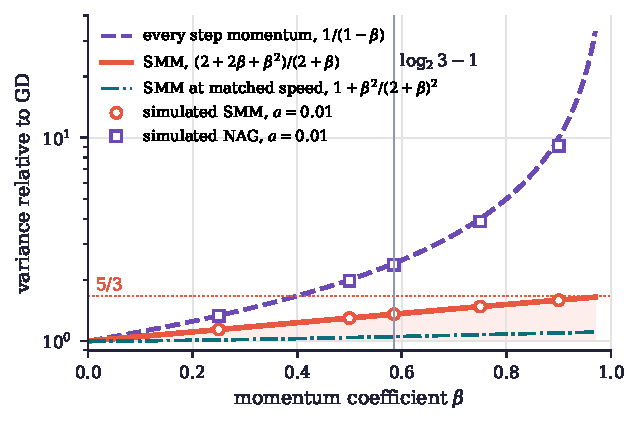
\includegraphics[width=0.85\textwidth]{figures/ch7_amplification.pdf}
  \caption{Slow mode variance amplification relative to gradient descent at the
  same step, as a function of the momentum coefficient (log scale). Dashed:
  every step momentum, $1/(1-\beta)$. Solid: \smmdet,
  $(2+2\beta+\beta^2)/(2+\beta)$, bounded by $5/3$ (dotted); the shaded band lies between $1$ and this curve.
  Dash dotted: \smmdet\ at matched speed, $1+\beta^2/(2+\beta)^2$ (\cref{prop:ch7:matched}).
  Markers: simulated
  ratios at $a=0.01$. The vertical line marks $\beta=\lt-1$.}
  \label{fig:ch7:amplification}
\end{figure}

\section{Beyond period two: the gain weight theorem}\label{sec:ch7:gainweight}

\Cref{prop:ch7:matched} compared \smmdet\ with gradient descent at matched speed
and found a small penalty, $1+\beta^2/(2+\beta)^2$. Is that penalty an accident
of the particular schedule, or would some other pattern of injections, of
period three or four, or with injection on several residues, beat gradient
descent? This is problem P6 of \cref{chap:open}. The answer is no, and the
reason is a single structural fact: in any first order method the noise enters
exactly where the gradient enters.

\paragraph{Setting.} Fix a period $p$ and a memory length $K$. On one
eigendirection of a quadratic, with $a=\alpha\lambda$ and state
$z_t=(e_t,\dots,e_{t-K+1})$, a \emph{linear periodic first order method}
evaluates at step $t$ (with residue $j=t\bmod p$) a gradient at an
extrapolated point $y_t=\gamma_j\cdot z_t$ and updates
\begin{equation}\label{eq:ch7:general}
  e_{t+1}=\delta_j\cdot z_t-h_j\bigl(a\,y_t+\alpha\,\xi_t\bigr),
\end{equation}
with fixed vectors $\gamma_j,\delta_j\in\R^K$ and step multipliers
$h_j>0$, where $\xi_t$ is the gradient noise. Consistency requires that
constants are preserved when the gradient vanishes, $\delta_j\cdot\iota=\gamma_j\cdot\iota=1$,
where $\iota=(1,\dots,1)$. Gradient descent, heavy ball\index{heavy ball}, Nesterov\index{Nesterov acceleration} at every
step, \smmdet, cyclic step\index{cyclic step sizes} sizes, and momentum\index{momentum} applied on any subset of the
residues modulo $p$ are all of this form.
Write $B(a)=B_0+aB_1+O(a^2)$ for the product of the $p$ step matrices over one period, and assume the method is \emph{stable at $a=0$}: the eigenvalue
$1$ of $B_0$, with right eigenvector $\iota$, is simple, and all other
eigenvalues of $B_0$ lie strictly inside the unit disc.

\begin{definition}[Gains]\label{def:ch7:gains}
Let $w$ be the left eigenvector of $B_0$ for the eigenvalue $1$, normalized so
that $w\cdot\iota=1$. The \emph{gain} $c_i$ of the gradient evaluated at
residue $i$ is the total long run effect, at $a=0$, of a unit injection
$-h_i$ into $e$ at that step, measured in the slow coordinate $w\cdot z$:
$c_i=h_i\,w\cdot\Pi_iu_1$, where $u_1$ is the first unit vector and $\Pi_i$ the product of the step matrices at $a=0$ from the step after $i$ to the end of the period. Put $M=\sum_{i=1}^pc_i$.
\end{definition}

The proof of part (i) of the theorem below shows that, whatever the sign of $M$, the period product has the eigenvalue $1-Ma+O(a^2)$, so $M\ge0$ is necessary for stability at small $a>0$. We assume $M>0$; this holds whenever all gains are positive, as for every method listed above with $\beta\in[0,1)$.

For gradient descent $c=1$; for every step momentum $c=1/(1-\beta)$, since a
unit impulse is carried forward with weights $1,\beta,\beta^2,\dots$; for
\smmdet\ the gains are $(1+\beta,\,1)$, because the gradient taken at a descent
step also enters the next extrapolation.

\begin{theorem}[Gain weight theorem]\label{thm:ch7:gainweight}\index{gain weight theorem}
For a linear periodic first order method \eqref{eq:ch7:general} that is stable at $a=0$ and has $M>0$, with
uncorrelated noise of variance $\sigma^2$, as $a\to0$:
\begin{enumerate}[label=(\roman*),leftmargin=2em]
\item the per step contraction of the slow mode is $1-(M/p)\,a+O(a^2)$;
\item the phase averaged stationary variance of $e_t$ is
  $\alpha^2\sigma^2\,\dfrac{\sum_ic_i^2}{2Ma}\,(1+o(1))$;
\item consequently the noise floor relative to gradient descent run at the same
  slow mode speed, step $(M/p)\alpha$, is
  \begin{equation}\label{eq:ch7:F}
    \mathcal F=\frac{p\sum_{i=1}^pc_i^2}{\bigl(\sum_{i=1}^pc_i\bigr)^2}\;\geq\;1,
  \end{equation}
  with equality if and only if all gains are equal.
\end{enumerate}
\end{theorem}

\begin{proof}
Let $s_t=w\cdot z_t$ at the start of each period. Since $w$ is a left
eigenvector of $B_0$, $s$ is unchanged by $B_0$, and over one period
\[
  s_{t+p}=s_t+a\,w\cdot B_1z_t-\alpha\sum_{i=1}^p c_i\,\xi_{t+i-1}+O(a\alpha)\,\|\xi\|,
\]
where the noise coefficients are the gains by \cref{def:ch7:gains}. The key
observation is that the deterministic term has the same coefficients. The
gradient enters \eqref{eq:ch7:general} through $h_j(a\,y_t+\alpha\xi_t)$,
so replacing $\alpha\xi_t$ by $a\,y_t$ shows that $a\,w\cdot B_1z_t=-a\sum_i
c_i\,y_{t+i-1}+O(a^2)\|z\|$. On the slow manifold $z\approx s\iota$ we have
$y\approx s$, because $\gamma_j\cdot\iota=1$, and therefore
$w\cdot B_1\iota=-M$. Simple eigenvalue perturbation now gives the
eigenvalue $1-Ma+O(a^2)$ of $B(a)$ for one period, which is (i).

Decompose $z_t=s_t\iota+f_t$ with $w\cdot f_t=0$. The fast part $f$ obeys a
recursion whose matrix is a perturbation of $B_0$ restricted to the complement
of $\iota$, which has spectral radius below $1$, so $f$ has stationary
variance $O(\alpha^2\sigma^2)$ uniformly in small $a$. The slow part satisfies
$s_{t+p}=(1-Ma)s_t+\eta_t+r_t$, where $\eta_t=-\alpha\sum_ic_i\xi_{t+i-1}$ has
variance $\alpha^2\sigma^2\sum_ic_i^2$ and is independent across periods, and
the remainder $r_t$ collects terms of order $a\,f_t$ and $a\alpha\,\xi$. Hence
$\Var(s)=\alpha^2\sigma^2\sum_ic_i^2/(1-(1-Ma)^2)\,(1+o(1))
=\alpha^2\sigma^2\sum_ic_i^2/(2Ma)\,(1+o(1))$. Since $e_t=s_t+(f_t)_1$ and
$|\Cov(s_t,(f_t)_1)|\le(\Var s\,\Var f)^{1/2}=O(\alpha^2\sigma^2a^{-1/2})$, the variance of
$e_t$ at every phase is $\Var(s)(1+o(1))$, which gives (ii).

Gradient descent with step $h\alpha$ has $c=h$, $M=h$ and variance
$\alpha^2\sigma^2h/(2a)$, and its slow mode contraction per step is $1-ha$.
Matching speeds means $h=M/p$, and the ratio of (ii) to
$\alpha^2\sigma^2(M/p)/(2a)$ is \eqref{eq:ch7:F}. The inequality is Cauchy and
Schwarz, $(\sum c_i)^2\le p\sum c_i^2$, with equality exactly when the $c_i$
are equal.
\end{proof}

\begin{corollary}[No schedule beats gradient descent in the slow mode]
\label{cor:ch7:nobeat}
Among all linear periodic first order methods that are stable at $a=0$ and have $M>0$, none has a lower slow
mode noise floor\index{noise floor} than gradient descent at matched speed. Every step heavy ball
and every step Nesterov attain equality, $\mathcal F=1$, which recovers the
equivalence of momentum SGD and SGD with a rescaled step at small step
sizes~\cite{yuan2016}. Switching MM\index{Switching MM} has $\mathcal F=2((1+\beta)^2+1)/(2+\beta)^2
=1+\beta^2/(2+\beta)^2$, recovering \cref{prop:ch7:matched}.
\end{corollary}

The theorem answers P6 negatively, and it also explains what the parity
schedule buys. Momentum in this regime is never free and never harmful at
matched speed: it simply buys speed at the price of noise in exact proportion,
provided all gradients receive the same weight. A schedule that weights
gradients unequally pays a Cauchy and Schwarz penalty. \smmdet\ weights its two
gradients in the ratio $1+\beta$ to $1$, which is why its penalty is small; a
cyclic step schedule $(1,3)$ weights them $1$ to $3$ and pays $\mathcal
F=5/4$. What parity switching achieves is not a better tradeoff but a
\emph{bounded} one: the speed multiplier $M/p=(2+\beta)/2$ never exceeds $3/2$ and the penalty $\mathcal F=1+\beta^2/(2+\beta)^2$ never exceeds $10/9$, so the floor, $\mathcal F M/p=V(\beta)$, never exceeds $5/3$ of gradient descent at the same step,
whatever $\beta$.

\Cref{tab:ch7:gainweight} checks the theorem against exact solutions of the
periodic Lyapunov equation for a range of schedules, and
\cref{fig:ch7:gainweight} shows the convergence of the exact matched speed
ratio to $\mathcal F$ as $a\to0$ (script \texttt{ch7\_gainweight.py}).

\begin{table}[tbp]
\centering\small
\caption{Gains, predicted floor factor $\mathcal F$ of \eqref{eq:ch7:F}, and
the exact matched speed ratio from the periodic Lyapunov equation at
$a=10^{-2}$ and $a=10^{-4}$. ``$p=3$, NAG at $\{2\}$'' injects Nesterov momentum
only at residue $2$ modulo $3$, and so on; $\beta_0=\lt-1$.}
\label{tab:ch7:gainweight}
\footnotesize
\setlength{\tabcolsep}{3pt}
\begin{tabular}{@{}lcccc@{}}
\toprule
Schedule & gains $c_i$ & $\mathcal F$ & $a=10^{-2}$ & $a=10^{-4}$ \\
\midrule
gradient descent & $1$ & $1$ & $1.0000$ & $1.0000$ \\
NAG every step, $\beta_0$ & $2.409$ & $1$ & $0.9773$ & $0.9998$ \\
NAG every step, $0.9$ & $10$ & $1$ & $0.8739$ & $0.9986$ \\
\smmdet, $\beta_0$ & $1.585,\ 1$ & $1.0512$ & $1.0466$ & $1.0512$ \\
\smmdet, $0.9$ & $1.9,\ 1$ & $1.0963$ & $1.0902$ & $1.0963$ \\
cyclic steps $(1,3)$ & $1,\ 3$ & $1.2500$ & $1.2570$ & $1.2501$ \\
$p=3$, NAG $\{2\}$, $\beta_0$ & $1,\ 1.585,\ 1$ & $1.0532$ & $1.0500$ & $1.0532$ \\
$p=3$, HB $\{1,2\}$, $0.9$ & $2.71,\ 1.9,\ 1$ & $1.1395$ & $1.1377$ & $1.1395$ \\
$p=4$, NAG $\{1,2,3\}$, $\beta_0$ & $2.13,\,1.93,\,1.58,\,1$ & $1.0663$ & $1.0561$ & $1.0662$ \\
$p=4$, NAG $\{2,3\}$, $0.9$ & $1,\,2.71,\,1.9,\,1$ & $1.1859$ & $1.1770$ & $1.1859$ \\
\bottomrule
\end{tabular}
\end{table}

\begin{figure}[tbp]
\centering
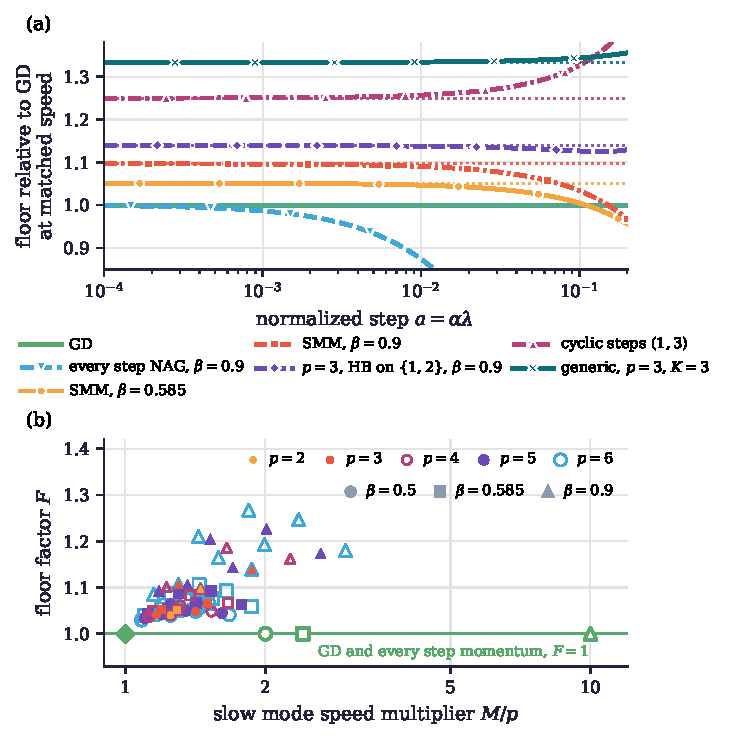
\includegraphics[width=\textwidth]{figures/ch7_gainweight.pdf}
\caption{The gain weight theorem. (a) Exact noise floor relative to gradient
descent at matched speed, from the periodic Lyapunov equation, against
$a=\alpha\lambda$, for six of the schedules of \cref{tab:ch7:gainweight} and for a period three schedule with three term memory and unrelated coefficients ($\mathcal F=1.333$); dotted lines are the limits $\mathcal F$. (b) The floor
factor $\mathcal F$ against the speed multiplier $M/p$ for all injection
subsets of periods $2$ to $6$ (larger markers for longer periods) and three values of $\beta$; only gradient
descent and every step momentum reach $\mathcal F=1$.}
\label{fig:ch7:gainweight}
\end{figure}

\section{The best period two ratio}\label{sec:ch7:pareto}

On quadratics \smmdet\ is the cyclic schedule with steps $h_1=\alpha$ and
$h_2=(1+\beta)\alpha$ (\cref{thm:smmquad}); in this section $h_1\le h_2$ denote absolute steps, not multiples of $\alpha$. Problem S3 asks which ratio
$r=h_2/h_1$ is best when both the deterministic rate and the noise floor\index{noise floor} matter.
For period two schedules both quantities depend on the ratio through a single
number,
\[
  G(r)=\frac{(1+r)^2}{4r}\ \geq1,
\]
and the tradeoff can be solved exactly.

\begin{proposition}[Rate and noise for period two steps]\label{prop:ch7:pareto}
Let the spectrum be $[\mu,L]$ with $\kappa=L/\mu$, and consider cyclic gradient
steps $h_1,h_2$ with ratio $r=h_2/h_1\ge1$.
\begin{enumerate}[label=(\roman*),leftmargin=2em]
\item The slow mode noise floor at matched speed is $N=2(h_1^2+h_2^2)/(h_1+h_2)^2
  =2-1/G(r)$.
\item For fixed $r$ with $G(r)\le G_{\mathrm{ch}}(\kappa)=2(\kappa+1)^2/(\kappa^2+6\kappa+1)$, the smallest possible worst case two step contraction over
  $[\mu,L]$ is
  \[
    R^*(r)=1-\frac{4\kappa\,G(r)}{(\kappa+1)^2},
  \]
  attained when the steps are scaled so that $h_1+h_2=4G(r)/(\mu+L)$.
  For $G(r)>G_{\mathrm{ch}}(\kappa)$ the smallest worst case contraction exceeds that of the Chebyshev ratio.
\item Consequently the Pareto frontier between rate and noise floor is
  $R=1-4\kappa/((2-N)(\kappa+1)^2)$ for $1\le N\le N_{\mathrm{ch}}(\kappa)$, where
  $N_{\mathrm{ch}}=(3\kappa^2+2\kappa+3)/(2(\kappa+1)^2)$ is the noise floor of
  the two step Chebyshev\index{Chebyshev step sizes} schedule, whose ratio tends to $(1+\sqrt2)^2=5.83$ and
  whose floor tends to $3/2$ as $\kappa\to\infty$.
\end{enumerate}
\end{proposition}

\begin{proof}
(i) is \eqref{eq:ch7:F} with $c=(h_1,h_2)$, and $2(h_1^2+h_2^2)/(h_1+h_2)^2
=2-4h_1h_2/(h_1+h_2)^2=2-1/G$. For (ii), the two step polynomial
$\Phi(\lambda)=(1-h_1\lambda)(1-h_2\lambda)$ satisfies $\Phi(0)=1$ and has minimum
$1-G$ at $\lambda_m=(h_1+h_2)/(2h_1h_2)$, so it can be written as
$\Phi(\lambda)=1-G+G(\lambda/\lambda_m-1)^2$. Its maximum over $[\mu,L]$ is at an
endpoint, and $\max\bigl((\mu/\lambda_m-1)^2,(L/\lambda_m-1)^2\bigr)$ is
minimized over $\lambda_m$ by $\lambda_m=(\mu+L)/2$, with value
$((\kappa-1)/(\kappa+1))^2$. Hence the endpoint maximum is at least
$1-G+G((\kappa-1)/(\kappa+1))^2=1-4\kappa G/(\kappa+1)^2$, with equality at
$\lambda_m=(\mu+L)/2$, i.e. $h_1+h_2=4G/(\mu+L)$.
At this scaling the interior minimum contributes $|1-G|=G-1$, and $G-1\le1-4\kappa G/(\kappa+1)^2$ exactly when $G\le G_{\mathrm{ch}}$, the two values being equal at the Chebyshev point $G=G_{\mathrm{ch}}$; since the endpoint bound holds for every scaling, this proves (ii) for such $G$.
For $G>G_{\mathrm{ch}}$ no scaling produces the two step Chebyshev polynomial~\cite{young1953,golub1961}, which is the unique minimizer of the worst case over $[\mu,L]$ among quadratic polynomials with value $1$ at $0$, so the worst case exceeds that of the Chebyshev ratio.
(iii) follows by eliminating $G=1/(2-N)$ for $G\le G_{\mathrm{ch}}$; beyond the Chebyshev point a larger ratio is worse than the Chebyshev ratio in both criteria.
\end{proof}

Every ratio between $1$ and the Chebyshev ratio $r_{\mathrm{ch}}(\kappa)$ is therefore on the frontier once its steps are scaled correctly, larger ratios being dominated by the Chebyshev ratio in both criteria, and the question becomes where on the frontier one wants to be.
The SMM ratio
$1+\beta$ gives $G=(2+\beta)^2/(4(1+\beta))=1.0540$ and $N=1.0512$: a $5.4$
percent gain in the rate exponent over optimally tuned gradient descent for a
$5.1$ percent rise in the noise floor. The Chebyshev ratio gains up to a factor
$2$ in the exponent but pays a floor up to $1.5$. The optimal scaling for the
SMM ratio is $\alpha L=4G\kappa/((2+\beta)(\kappa+1))$, which tends to
$(2+\beta)/(1+\beta)=1.631$; at the conventional $\alpha=1/L$ the method is not
on the frontier, and its per step factor at $\kappa=100$ is $0.9871$ against
$0.9791$ when optimally scaled. \Cref{fig:ch7:pareto} draws the frontier. The
SMM ratio coincides with the Chebyshev ratio only at $\kappa_0=1.94$; for
larger $\kappa$ it sits close to the gradient descent end of the frontier,
which is the noise conservative end.

\begin{figure}[tbp]
\centering
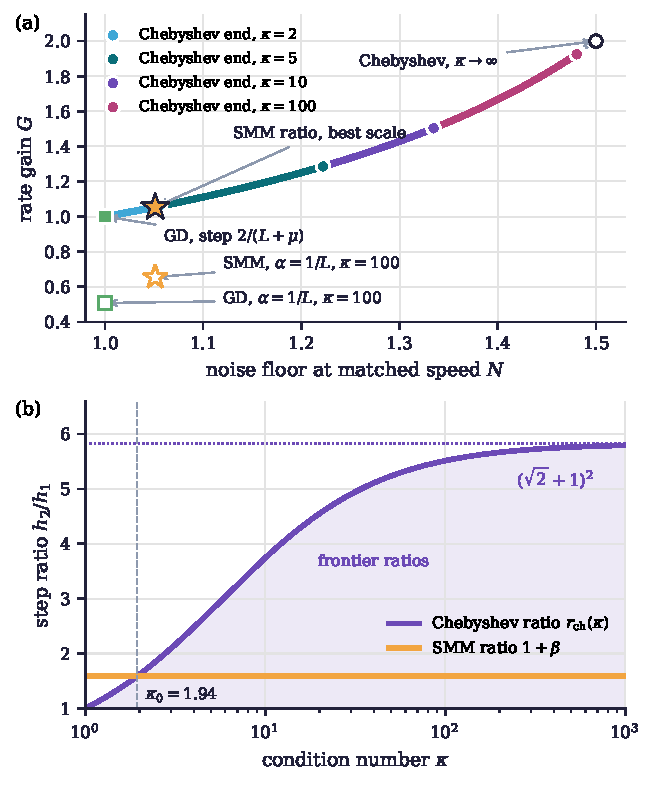
\includegraphics[width=\textwidth]{figures/ch7_pareto.pdf}
\caption{(a) The rate gain $G$ against the noise floor $N$ at matched speed for period two schedules. By \cref{prop:ch7:pareto}(i) all frontiers lie on the curve $G=1/(2-N)$ and differ only in where they end, at the Chebyshev schedule for each $\kappa$. The star is the SMM ratio at its best scale, the open markers SMM and gradient descent at $\alpha=1/L$ and $\kappa=100$, and the filled square gradient descent at step $2/(L+\mu)$. The frontier ends for $\kappa=2,5,10,100$ lie in that order along the curve: the first under the star, the others at the dots. (b) The Chebyshev ratio $r_{\mathrm{ch}}(\kappa)$, rising to $(1+\sqrt2)^2$, and the SMM ratio $1+\beta$; they cross at $\kappa_0=1.94$.}
\label{fig:ch7:pareto}
\end{figure}

\section{Multiplicative noise}\label{sec:ch7:multiplicative}

Additive noise is the simplest model. In least squares, and more generally in
stochastic gradient methods with sampled data, the noise also multiplies the
error: the sampled curvature fluctuates. Problem S2 asks whether the
conclusions survive. Consider on one eigendirection the oracle
\[
  g(y)=(\lambda+\eta_t)\,e_y+\xi_t,
\]
with $\eta_t,\xi_t$ independent of the past, mean zero, uncorrelated with each
other, $\Var(\alpha\eta_t)=\omega^2$ and $\Var\xi_t=\sigma^2$. Two scalings are
natural: the least squares scaling $\omega^2=\vartheta a^2$, in which the
relative curvature noise\index{multiplicative noise} $\vartheta=\Var(x^2)/(\E x^2)^2$ is fixed ($\vartheta=2$
for a Gaussian regressor), and the diffusive scaling $\omega^2=\epsilon a$.

\begin{proposition}[Multiplicative noise]\label{prop:ch7:mult}
For \smmdet\ the second moments obey a closed linear recursion: with
$\nu_1=(1-a)^2+\omega^2$ and $\nu_2=(1-(1+\beta)a)^2+(1+\beta)^2\omega^2$,
the stationary second moment at even times is
$\alpha^2\sigma^2(\nu_1(1+\beta)^2+1)/(1-\nu_1\nu_2)$, finite if and only
if $\nu_1\nu_2<1$. As $a\to0$:
\begin{enumerate}[label=(\roman*),leftmargin=2em]
\item under the least squares scaling the slow mode ratio to gradient descent is
  unchanged, $(2+2\beta+\beta^2)/(2+\beta)$, for every $\vartheta$;
\item under the diffusive scaling, for any linear periodic method that is stable at $a=0$ and has $M>0$, with
  gains $c_i$, $a\,\E e^2\to\alpha^2\sigma^2\sum_ic_i^2/(2M-\epsilon\sum_ic_i^2)$,
  so the method is mean square stable for small $a$ exactly when
  $\epsilon<\epsilon^*=2M/\sum_ic_i^2$.
\end{enumerate}
\end{proposition}

\begin{proof}
For \smmdet\ the two step recursion of \cref{thm:smmvar} holds with each factor
$(1-ha)$ replaced by $(1-h(a+\alpha\eta))$; squaring and taking expectations,
the cross terms vanish by independence and the factors $\nu_1,\nu_2$
appear, which gives the closed form and the stability condition. Statement (i)
follows because $\omega^2=\vartheta a^2$ changes $\nu_1,\nu_2$ only at order
$a^2$, which does not affect the leading term of $1-\nu_1\nu_2$. For (ii),
repeat the slow coordinate argument of \cref{thm:ch7:gainweight}: the
multiplicative noise contributes to $s$ a term $-\alpha\sum_ic_i\eta_{t+i}s$ per
period, of variance $\epsilon a\sum_ic_i^2\,s^2$, so the stationary second
moment satisfies $\E s^2=(1-2Ma+\epsilon a\sum c_i^2)\E s^2+\alpha^2\sigma^2\sum
c_i^2+o(a)\E s^2$, which gives the stated limit and threshold.
\end{proof}

The threshold $\epsilon^*=2M/\sum c_i^2$ is a clean measure of robustness to
curvature noise. It is $2$ for gradient descent, $2(1-\beta)$ for every step
momentum\index{momentum}, $0.830$ at $\beta=\beta_0=\lt-1$ and $0.2$ at $\beta=0.9$, and
$2(2+\beta)/((1+\beta)^2+1)$ for \smmdet, which is $1.472$ at $\beta_0$ and
$1.258$ at $\beta=0.9$ and never falls below $6/5$. So under curvature noise the
parity schedule is markedly more robust than every step momentum, by a factor
that grows without bound as $\beta\to1$.
At matched slow mode speed the comparison changes, as it did for the variance: gradient descent with step $(M/p)\alpha$ has $\epsilon^*=2p/M$, and the ratio of the two thresholds is $M^2/(p\sum_ic_i^2)=1/\mathcal F\le1$.
Away from the slow mode the picture is
more nuanced. The uniform bound $5/3$ does not survive large multiplicative
noise at large $a$: at $\beta=\beta_0$ \smmdet\ remains mean square stable at
$a=1$ only for $\vartheta<0.566$, and above that it is not mean square stable at $a=1$, where gradient descent still is for $\vartheta<1$; but every step Nesterov\index{Nesterov acceleration} loses
stability earlier at every $\vartheta$ we examined (\cref{fig:ch7:multiplicative},
script \texttt{ch7\_multiplicative.py}, with Monte Carlo checks agreeing with the
closed forms to three digits).

\begin{figure}[tbp]
\centering
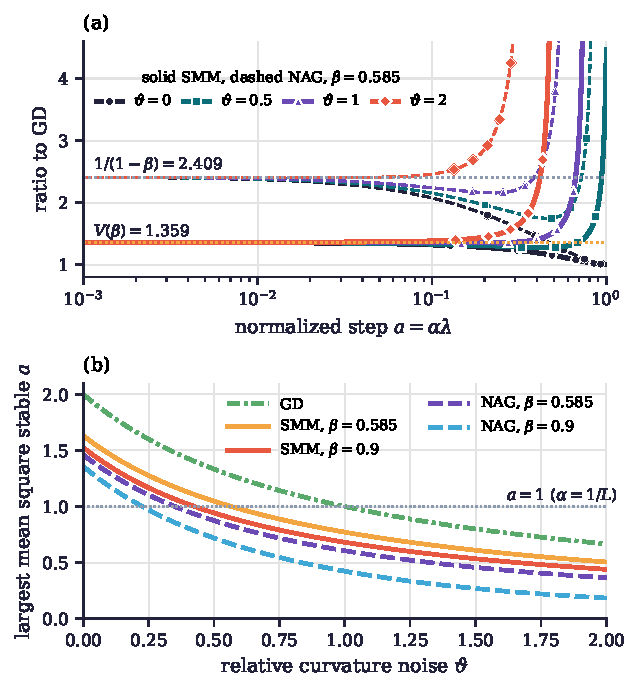
\includegraphics[width=\textwidth]{figures/ch7_multiplicative.pdf}
\caption{Multiplicative noise under the least squares scaling. (a) Stationary
second moment relative to gradient descent against $a$, for \smmdet\ (solid)
and every step Nesterov (dashed) at $\beta=0.585$ and several $\vartheta$; the
slow mode limits $V(\beta)=1.359$ and $1/(1-\beta)=2.409$ are marked. (b) The
largest mean square stable $a$ as a function of $\vartheta$; \smmdet\ is stable
on a larger range than every step Nesterov at the same $\beta$.}
\label{fig:ch7:multiplicative}
\end{figure}

\section{The experiments}\label{sec:ch7:experiments}

We now describe experiments with SMM and then reconcile them with the exact theory in \cref{sec:ch7:reconcile}. The experiments were designed before that theory was available. The numbers and figures below come from a rerun for this book: the script \texttt{ch7\_experiments.py} runs the experiments, and the scripts \texttt{ch7\_experiments\_fig.py} and \texttt{ch7\_noisefig.py} draw the figures.

\subsection{Setup and baselines}

\smmdet\ and, where indicated, \smmstate\ (\cref{alg:smmdet,alg:smmstate}) were
compared with gradient descent at step $1/L$; with heavy ball\index{heavy ball} and Nesterov\index{Nesterov acceleration} at
their textbook strongly convex tunings~\cite{polyak1987,nesterov2004}, which
need $\mu$ (heavy ball with $\alpha=4/(\sqrt L+\sqrt\mu)^2$ and
$\beta=\bigl((\sqrt L-\sqrt\mu)/(\sqrt L+\sqrt\mu)\bigr)^2$, Nesterov with
$\alpha=1/L$ and $\beta=(\sqrt L-\sqrt\mu)/(\sqrt L+\sqrt\mu)$); and with fixed
momentum\index{momentum} heavy ball and Nesterov at the four candidates
$\beta\in\{0.5,0.585,0.667,0.9\}$ of \cref{tab:ch6:candidates}. The fixed
momentum row at $\beta=0.585$ is the every step analogue of \smmdet\ and
isolates the parity schedule. Adam~\cite{kingma2015} at its defaults
($\beta_1=0.9$, $\beta_2=0.999$, $\epsilon=10^{-8}$, step $1/L$) served as a
reference from a different family. Every method received $L$.
Fixed momentum Nesterov is the update $y_t=x_t+\beta(x_t-x_{t-1})$, $x_{t+1}=y_t-\alpha\nabla f(y_t)$ at every step, and fixed heavy ball the update of \cref{sec:ch7:ar2}, both with $\alpha=1/L$; the frequency ablation adds injection at random steps, each step injecting independently with probability $\tfrac12$. \smmstate\ runs \cref{alg:smmstate} with $\rho_{\mathrm{thr}}=0.356$, reference value $f_{\mathrm{ref}}=f^\ast$, the minimum of the objective, and $\epsilon=10^{-12}$.

The test problems were random quadratics $f(x)=\tfrac12x^\top Ax$ in dimension $d=25$, with eigenvalues geometrically spaced in $[1,\kappa]$, a random orthogonal eigenbasis and $x_0$ drawn from $N(0,I)$; and $\ell_2$ regularized logistic regression on the Breast Cancer Wisconsin data~\cite{wolberg1995} ($n=569$ samples, $30$ standardized features, no intercept, penalty $0.05$), with initial weights drawn from $N(0,0.1^2I)$; there $\mu=0.05$ and $L=\lambda_{\max}(X^\top X/n)/4+0.05=3.370$ for the $n\times30$ data matrix $X$, so that $\kappa=L/\mu\approx67.4$. The count of a run is the first iteration at which the objective gap falls below the tolerance, and a run that has not reached the tolerance within the horizon $T$ counts as $T+1$. Means and standard errors are over $R$ seeded replicates: $R=20$ for the quadratic and logistic experiments, $R=30$ for the noise sweep and the minibatch test.

\subsection{Quadratic condition number sweep and frequency ablation}

\Cref{fig:ch7:ksweep} reports the mean number of iterations to reach an objective gap below $10^{-4}$ for $\kappa\in\{2,5,10,25,50,100\}$, with horizon $T=300$. At $\kappa=2$, \smmdet\ is the fastest method tested, with $4.85$ iterations on average. At $\kappa=5$ only every step Nesterov\index{Nesterov acceleration} at $\beta=0.5$ and at $\beta=0.585$ is clearly faster ($11.85$ and $12.6$ iterations against $15.95$); Nesterov at $\beta=0.667$ ties with \smmdet, and every step heavy ball\index{heavy ball} at these coefficients is slower. For $\kappa\ge10$ every step heavy ball and Nesterov at $\beta\in\{0.585,0.667\}$ beat it, by factors from about $1.1$ to $2.0$ at $\kappa=10$ and from $2.1$ to $2.9$ at $\kappa=25$. At $\kappa=50$ the coefficient $0.667$ is fastest in both forms, and only at $\kappa=100$ is fixed Nesterov at $\beta=0.9$ fastest. The nearly flat stretches of the fixed heavy ball curves reflect underdamping: when every normalized step exceeds $(1-\sqrt\beta)^2$, which holds for $\kappa<(1-\sqrt\beta)^{-2}$ (about $12$, $18$, $30$ and $380$ for the four candidates), both characteristic roots have modulus $\sqrt\beta$ whatever $a$, so the iteration count is set by $\beta$ rather than by the conditioning.

\begin{figure}[tbp]
  \centering
  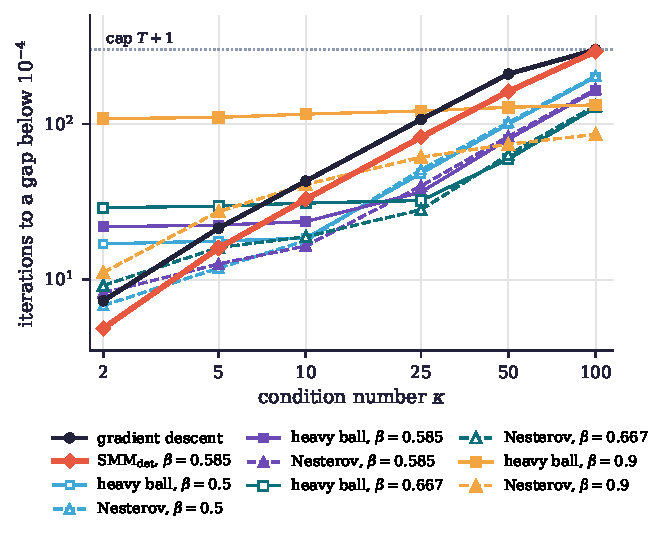
\includegraphics[width=\textwidth]{figures/ch7_ksweep.pdf}
  \caption{Fixed momentum baselines on random quadratics ($d=25$, $R=20$,
  $T=300$): mean iterations to an objective gap below $10^{-4}$ against the
  condition number. Heavy ball (squares, solid) and Nesterov (triangles,
  dashed) at the four candidate coefficients, gradient descent, and \smmdet.
  A run that has not reached the tolerance by $T$ counts as $T+1=301$ (dotted line); at $\kappa=100$ this cap censors $19$ of the $20$ gradient descent runs and $14$ of the $20$ \smmdet\ runs.}
  \label{fig:ch7:ksweep}
\end{figure}

\Cref{fig:ch7:ablation} isolates the schedule at $\beta=0.585$: injection at every step, at odd steps (\smmdet), at random steps with probability $\tfrac12$, and never. Without noise, parity does not help. Every step injection needs $16.45$ iterations at $\kappa=10$ against $32.85$ for parity, a ratio of $2.00$, and $167$ against $293$ at $\kappa=100$; there $14$ of the $20$ parity runs reach the horizon, so the parity count is censored, and continued to convergence (the script runs every instance for $3000$ steps) the parity schedule needs $318$ iterations, a ratio of $1.90$. Random injection lies between the two, closer to parity for $\kappa\ge10$. Only at $\kappa=2$, where all normalized steps are large and the period two polynomial $\rho(a)$ is small, does parity win. The ratios $2.00$ and $1.90$ are close to the slow mode prediction $m_{\mathrm{NAG}}/m_{\mathrm{SMM}}=1.86$ of \cref{cor:ch6:slow} and the discussion following it; \cref{chap:smm} makes the same check with more replicates.

\begin{figure}[tbp]
  \centering
  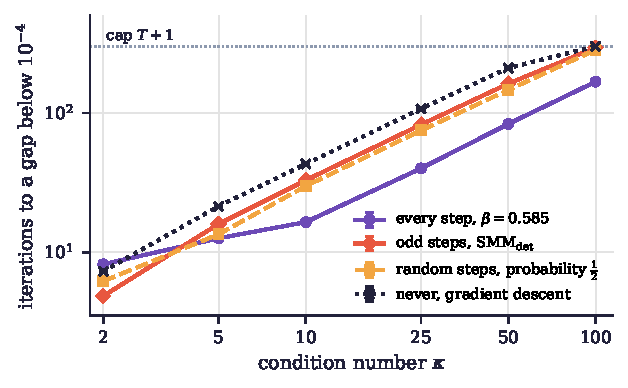
\includegraphics[width=\textwidth]{figures/ch7_ablation.pdf}
  \caption{Frequency ablation on random quadratics at fixed $\beta=0.585$
  ($d=25$, $R=20$, $T=300$): injection at every step, at odd steps (\smmdet),
  at random steps with probability $\tfrac12$, and never (gradient descent).
  Bars are standard errors. A run that has not reached the tolerance by $T$ counts as $301$ (dotted line), which censors most parity and gradient descent runs and half of the random injection runs at $\kappa=100$.}
  \label{fig:ch7:ablation}
\end{figure}

\subsection{Noise robustness}

The central experiment adds Gaussian noise of standard deviation $\sigma\in\{0,\allowbreak0.05,\allowbreak0.10,\allowbreak0.20,\allowbreak0.40\}$ to the gradients of random quadratics with $\kappa=25$, with the same noise draws for every method, and records the objective gap after $T=300$ steps (\cref{fig:ch7:noise,tab:noise}). At every positive noise level \smmdet\ has the lowest final gap among the inertial methods: at $\sigma=0.1$, $3.7\times10^{-3}$ against $5.0\times10^{-3}$ for every step Nesterov momentum\index{momentum} at the same $\beta$ and $1.1\times10^{-2}$ at $\beta=0.9$. Across the sweep every step Nesterov at $\beta=0.585$ is $29$ to $36$ percent worse than \smmdet, and $\beta=0.9$ about $2.5$ to $3$ times worse; heavy ball at the same coefficients is worse still. Gradient descent has the lowest gap of all at each positive $\sigma$, and \smmdet\ stays within $27$ percent of it.

\begin{figure}[tbp]
  \centering
  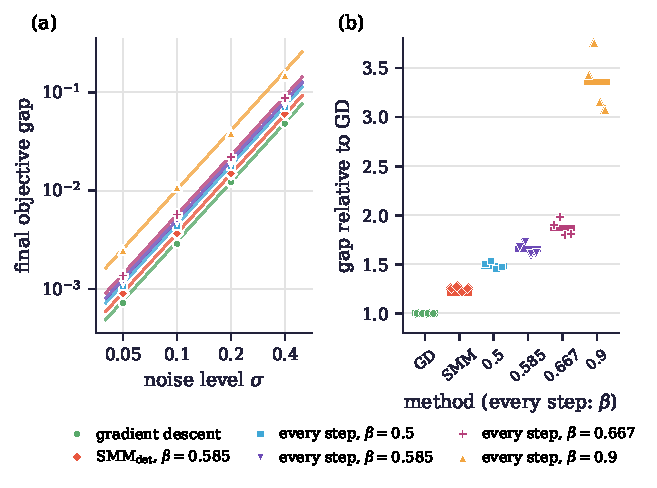
\includegraphics[width=\textwidth]{figures/ch7_noise.pdf}
  \caption{The noise robustness experiment of \cref{tab:noise}. (a) Final
  objective gap after $T=300$ steps against the noise level (points), with the
  stationary predictions of \eqref{eq:ch7:gd}, \cref{thm:smmvar} and \cref{prop:ch7:nag} summed
  over the spectrum (lines). (b) The gap relative to gradient descent for
  each method at the four positive noise levels (points), with the predicted ratios marked (bars). The every step rows use the Nesterov form.}
  \label{fig:ch7:noise}
\end{figure}

\begin{table}[tbp]
\centering
\caption{Noise robustness on random quadratics with $\kappa=25$ ($d=25$,
$T=300$, $R=30$): final objective gap, lower is better. A dagger marks the
lowest gap among inertial methods at each positive noise level; gradient
descent, which has no momentum, is lower still. ``every, $\beta$'' denotes
Nesterov momentum $\beta$ injected at every step, and ``HB, $\beta$'' heavy ball.}
\label{tab:noise}
\footnotesize
\setlength{\tabcolsep}{2.2pt}
\begin{tabular}{lccccc}
\toprule
Method & $\sigma=0$ & $0.05$ & $0.10$ & $0.20$ & $0.40$\\
\midrule
GD & $1.8\times10^{-11}$ & $7.2\times10^{-4}$ & $2.9\times10^{-3}$ & $1.2\times10^{-2}$ & $4.8\times10^{-2}$\\
every, $0.5$ & ${\approx}\,0$ & $1.1\times10^{-3}$ & $4.4\times10^{-3}$ & $1.8\times10^{-2}$ & $7.1\times10^{-2}$\\
every, $0.585$ & ${\approx}\,0$ & $1.2\times10^{-3}$ & $5.0\times10^{-3}$ & $2.0\times10^{-2}$ & $7.8\times10^{-2}$\\
\smmdet, parity & $1.1\times10^{-14}$ & $9.0\times10^{-4}\,^\dagger$ & $3.7\times10^{-3}\,^\dagger$ & $1.5\times10^{-2}\,^\dagger$ & $6.0\times10^{-2}\,^\dagger$\\
every, $0.667$ & ${\approx}\,0$ & $1.4\times10^{-3}$ & $5.7\times10^{-3}$ & $2.2\times10^{-2}$ & $8.7\times10^{-2}$\\
every, $0.9$ & ${\approx}\,0$ & $2.5\times10^{-3}$ & $1.1\times10^{-2}$ & $3.8\times10^{-2}$ & $1.5\times10^{-1}$\\
HB, $0.585$ & ${\approx}\,0$ & $1.5\times10^{-3}$ & $6.7\times10^{-3}$ & $2.6\times10^{-2}$ & $1.1\times10^{-1}$\\
HB, $0.9$ & $1.2\times10^{-12}$ & $6.3\times10^{-3}$ & $2.8\times10^{-2}$ & $1.1\times10^{-1}$ & $3.9\times10^{-1}$\\
\bottomrule
\end{tabular}
\end{table}

\subsection{Logistic regression and Adam}

On the regularized logistic regression (\cref{tab:ch7:logistic}, horizon $T=600$), fixed momentum\index{momentum} $\beta=0.667$ is fastest in both forms, with about $41$ iterations to a gap below $10^{-4}$; the Collatz coefficient at every step needs about $52$, \smmdet\ about $100$ and gradient descent $129$. Without noise, every step injection at a moderate fixed $\beta$ is the better choice. \Cref{fig:ch7:logistic} adds the tuned methods, which use $\mu$ and reach machine precision far sooner ($19.3$ and $29.0$ iterations to the tolerance for heavy ball and Nesterov), and \smmstate, whose rule fires at almost every step on this problem ($599.5$ of the $600$ steps on average), so that it follows every step Nesterov at $\beta=0.585$, with $53.0$ iterations. Adam, with $75.9$ iterations, lies between fixed Nesterov\index{Nesterov acceleration} at $\beta=0.9$ ($50.3$) and \smmdet. Adam keeps two moment vectors per coordinate where SMM, heavy ball\index{heavy ball} and Nesterov keep one extra vector; it needs neither $\mu$ nor a tuned coefficient, but on this problem every fixed momentum method except heavy ball at $\beta=0.9$ is faster.

\begin{table}[tbp]
\centering
\caption{Logistic regression on the Breast Cancer Wisconsin data (penalty $0.05$,
$\kappa\approx67.4$, $T=600$, $R=20$): iterations to a gap below $10^{-4}$ (mean
and standard error), observed speedup over gradient descent, and the slow mode
prediction of \cref{sec:ch7:reconcile}. An asterisk marks methods underdamped in
the slowest mode.}
\label{tab:ch7:logistic}
\begin{tabular}{lccc}
\toprule
Method & Iterations & Speedup & Predicted\\
\midrule
GD & $128.8\pm1.5$ & $1$ & $1$\\
HB, $\beta=0.5$ & $63.1\pm0.7$ & $2.04$ & $2.08$\\
HB, $\beta=0.585$ & $51.6\pm0.6$ & $2.50$ & $2.58$\\
HB, $\beta=0.667$ & $40.3\pm0.4$ & $3.20$ & $3.41$\\
HB, $\beta=0.9$ & $77.0\pm1.0$ & $1.67$ & $3.52^{*}$\\
NAG, $\beta=0.5$ & $64.1\pm0.7$ & $2.01$ & $2.05$\\
NAG, $\beta=0.585$ & $52.8\pm0.6$ & $2.44$ & $2.52$\\
NAG, $\beta=0.667$ & $41.9\pm0.5$ & $3.08$ & $3.28$\\
NAG, $\beta=0.9$ & $50.3\pm0.3$ & $2.56$ & $4.02^{*}$\\
\smmdet, $\beta=0.585$ & $99.7\pm1.2$ & $1.29$ & $1.30$\\
\bottomrule
\end{tabular}
\end{table}

\begin{figure}[tbp]
  \centering
  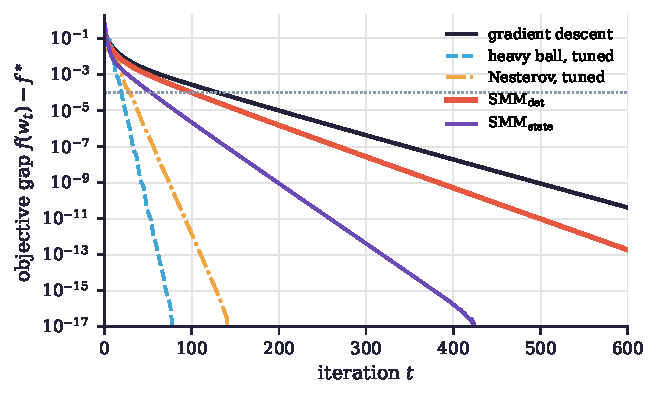
\includegraphics[width=\textwidth]{figures/ch7_logistic.pdf}
  \caption{Logistic regression (penalty $0.05$, $\kappa\approx67$, $T=600$, mean
  of $R=20$ runs): objective gap against iteration for gradient descent, tuned
  heavy ball and Nesterov, \smmdet\ and \smmstate; the dotted line is the tolerance $10^{-4}$.
  \smmstate\ injects at almost every step here and follows every step Nesterov at $\beta=0.585$.}
  \label{fig:ch7:logistic}
\end{figure}

\subsection{Minibatch stochastic gradients}

A more realistic test replaces the full logistic gradient by minibatch gradients with $|B|\in\{16,64,256\}$, the batches drawn without replacement and shared by all methods, keeping the step $1/L$ (\cref{tab:ch7:sgd,fig:ch7:sgd}). At $|B|=16$ every method that injects at every step, including tuned Nesterov\index{Nesterov acceleration}, reaches the tolerance $10^{-3}$ late or not at all: tuned Nesterov and Nesterov at $\beta=0.9$ in none of the $30$ runs, Nesterov at $\beta=0.585$ after $273$ iterations on average, with $2$ runs that never do. \smmdet\ is the only inertial method that reaches it reliably, in $135$ iterations, and gradient descent, with $118$, is faster still. As the batch grows the deterministic ranking returns: at $|B|=256$ tuned Nesterov is fastest with $21$ iterations. Among the every step Nesterov variants the default $\beta=0.9$ is never faster than the others: at $|B|=16$ it ties with tuned Nesterov, neither reaching the tolerance, and at $|B|=64$ and $256$ it is the slowest of the three.

\begin{table}[tbp]
\centering
\caption{Minibatch stochastic gradients on the logistic regression: iterations
to a gap below $10^{-3}$ (mean and standard error, $T=600$, $R=30$; a run that does not reach the tolerance within $T$ counts as $601$). A dagger
marks the best inertial method at each batch size; ``cap'' marks entries in which no run reached the tolerance.}
\label{tab:ch7:sgd}
\begin{tabular}{lccc}
\toprule
Method & $|B|=16$ & $|B|=64$ & $|B|=256$\\
\midrule
GD & $118.2\pm6.3$ & $77.7\pm1.5$ & $67.6\pm1.1$\\
NAG, tuned & $601\pm0$ (cap) & $36.5\pm2.3\,^\dagger$ & $21.2\pm0.2\,^\dagger$\\
NAG, $\beta=0.585$ & $272.7\pm30.7$ & $40.6\pm1.3$ & $29.3\pm0.5$\\
NAG, $\beta=0.9$ & $601\pm0$ (cap) & $113.5\pm14.7$ & $36.5\pm0.8$\\
\smmdet, $\beta=0.585$ & $135.2\pm11.2\,^\dagger$ & $62.7\pm1.7$ & $53.1\pm0.9$\\
\bottomrule
\end{tabular}
\end{table}

\begin{figure}[tbp]
  \centering
  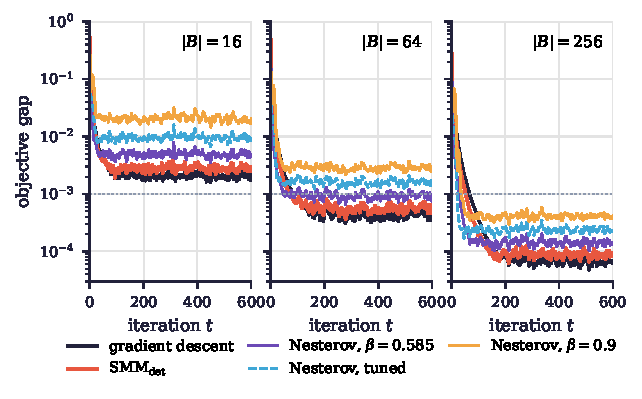
\includegraphics[width=\textwidth]{figures/ch7_sgd.pdf}
  \caption{Minibatch stochastic gradients on the logistic regression ($T=600$,
  mean of $R=30$ runs; the dotted line is the tolerance $10^{-3}$). In every panel the plateaus are ordered from gradient
  descent (lowest) through \smmdet, Nesterov at $\beta=0.585$ and tuned Nesterov
  to Nesterov at $\beta=0.9$ (highest).}
  \label{fig:ch7:sgd}
\end{figure}

In summary, read on their own, the experiments say the following: without noise, every step Nesterov momentum beats \smmdet\ at the same coefficient for $\kappa\ge5$, and every step heavy ball for $\kappa\ge10$; with noise, \smmdet\ has the lowest final gap among inertial methods and copes best with the smallest minibatch; and $0.585$ is a reasonable default among fixed momenta but not a universally optimal one, and nothing in the theory of this chapter singles it out.

\section{Reconciling the experiments with the exact theory}\label{sec:ch7:reconcile}

\paragraph{The noise floors.} The $\kappa=25$ experiment has $\alpha=1/25$ and
normalized steps $a_j=\lambda_j/25\in[0.04,1]$. After $T=300$ steps the
deterministic transient has decayed by at least $0.96^{300}<10^{-5}$, so by
\eqref{eq:ch7:gap} the final gap is essentially
$\tfrac12\sum_{j}\lambda_jV(a_j)$, with $V$ the exact stationary variance of the
method. For gradient descent this sum is $0.3055\,\sigma^2$, that is
$7.6\times10^{-4}$, $3.05\times10^{-3}$, $1.22\times10^{-2}$ and
$4.89\times10^{-2}$ at the four noise levels, against the measured
$7.2\times10^{-4}$, $2.9\times10^{-3}$, $1.22\times10^{-2}$ and $4.8\times10^{-2}$.
\Cref{tab:ch7:reconcile} does the same for the ratios to gradient descent.
The every step rows of \cref{tab:noise} use the Nesterov\index{Nesterov acceleration} form of every step momentum\index{momentum}, and its predictions match the data closely at all four coefficients; so do the much larger heavy ball\index{heavy ball} predictions for the two heavy ball rows.
The predicted ratio of every step Nesterov at $\beta=0.585$ to \smmdet\ is $1.65/1.21=1.36$, matching the observed $29$ to $36$ percent, and the predicted excess of \smmdet\ over gradient descent is $21$ percent, against the observed $22$ to $27$ percent.

\begin{table}[tbp]
\centering
\caption{Final gap relative to gradient descent in the $\kappa=25$ noise
experiment: prediction from the exact stationary variances summed over the
spectrum, and the range of measured ratios over the four positive noise levels
of \cref{tab:noise}.}
\label{tab:ch7:reconcile}
\begin{tabular}{lcc}
\toprule
Method & Predicted & Measured\\
\midrule
\smmdet, $\beta=0.585$ & $1.21$ & $1.22$ to $1.27$\\
NAG, $\beta=0.5$ & $1.49$ & $1.46$ to $1.54$\\
NAG, $\beta=0.585$ & $1.65$ & $1.61$ to $1.73$\\
NAG, $\beta=0.667$ & $1.87$ & $1.80$ to $1.98$\\
NAG, $\beta=0.9$ & $3.36$ & $3.07$ to $3.76$\\
HB, $\beta=0.585$ & $2.21$ & $2.14$ to $2.31$\\
HB, $\beta=0.9$ & $8.96$ & $8.02$ to $9.86$\\
\bottomrule
\end{tabular}
\end{table}

\paragraph{Why gradient descent wins the noise table.} That gradient descent has
the lowest final gap at every positive $\sigma$ is forced by the theory.
At a fixed step every inertial method considered has stationary variance at least that of gradient descent on every eigendirection with $a\le1$: for \smmdet\ by \cref{prop:ch7:uniform}; for Nesterov because $V_{\mathrm{NAG}}-V_{\mathrm{GD}}=2\beta(1+\beta)(1-a)^2\alpha^2\sigma^2/\bigl(a(2-a)(1-\beta+a\beta)(2(1+\beta)-a(1+2\beta))\bigr)\ge0$, an identity checked by \texttt{ch7\_extra.py}; and for heavy ball because its ratio $(1+\beta)(2-a)/\bigl((1-\beta)(2(1+\beta)-a)\bigr)$ is at least $1$ whenever $a\le1+\beta$.
The dagger in \cref{tab:noise} is therefore to be read with the
gradient descent row: \smmdet\ gives up little of the quietness of gradient
descent while being faster than it without noise, and every step momentum gives
up much more.

\paragraph{The minibatch test.} The noise of a minibatch gradient is neither
additive nor isotropic, but the plateaus of \cref{fig:ch7:sgd} are ordered exactly as the
slow mode amplifications: gradient descent ($1$), \smmdet\ ($1.36$), Nesterov at
$\beta=0.585$ ($2.41$), tuned Nesterov, whose coefficient at $\kappa=67.4$ is
$0.783$ with $1/(1-\beta)=4.60$, and Nesterov at $\beta=0.9$ ($10$). The
iteration counts mix this ordering with speed (\cref{rem:ch7:budget}). At
$|B|=16$ the mean plateaus of all methods lie near or above $10^{-3}$, so the
count is a first passage time of a fluctuating gap below a level close to the
floor; the lower the floor, the sooner the crossing, which favours gradient
descent and \smmdet. At $|B|=256$ all floors lie well below the tolerance and
speed decides.

\paragraph{The deterministic speedups.} In the slowest mode of the logistic
regression, $a=1/67.4$, the predicted speedup over gradient descent is
$\log r/\log(1-a)$, where $r$ is the per step factor of the method: the spectral
radius of its companion matrix, or $|\rho(a)|^{1/2}$ for \smmdet.
For \smmdet\ the prediction, $1.296$, agrees within $0.3$ percent with the observed ratio of the mean counts, $128.80/99.65=1.293$; for the overdamped heavy ball and Nesterov runs, $\beta\le0.667$, prediction and observation agree within seven percent, the prediction always
slightly optimistic, as expected of a count that includes the initial
transient. Only the underdamped runs at $\beta=0.9$ deviate, since their
oscillatory convergence is not governed by the asymptotic rate alone.

In short, the exact theory confirms the qualitative findings, explains their magnitudes, and adjusts one reading: in the slow modes SMM is not more efficient than gradient descent under noise, although over the whole spectrum of the $\kappa=25$ experiment its floor, $1.21$ times that of gradient descent at the same step, is below the $1.42$ of gradient descent run at the same slow mode speed; it is much quieter than every step momentum at the same $\beta$, and its noise behaviour is almost insensitive to $\beta$.

\section{Practical guidance and limitations}\label{sec:ch7:guidance}

If gradients are exact and $\mu$ is available, a tuned accelerated method is
the right tool; SMM is not accelerated. If gradients are exact and $\mu$ is
unknown, every step momentum\index{momentum} at a moderate fixed coefficient such as $0.585$ or
$0.667$ is faster than SMM by a factor near $m_{\mathrm{NAG}}/m_{\mathrm{SMM}}$.
If gradients are noisy at an unknown level, \smmdet\ is a safe default: its
floor is within $5/3$ of that of gradient descent at the same step for every
$\beta<1$ and on every eigendirection, it is stable at step $1/L$ for every
$\beta<1$, and at the Collatz coefficient it is about $29$ percent faster than
gradient descent in the slow modes; if only the floor at a given slow mode speed matters, gradient descent with a slightly longer step is slightly better in the slow eigendirections but worse over the whole spectrum ($1.42$ against $1.21$ in the $\kappa=25$ experiment).
If per coordinate preconditioning is affordable, Adam is an alternative that needs no $\mu$, although in the logistic experiment it was slower than every step momentum at a moderate coefficient. Iterate
averaging~\cite{polyak1992} or a decreasing step lowers the floor of any of
these methods; our comparisons are for a constant step.

The exact noise theory covers quadratics, with additive noise independent across iterations (\cref{thm:smmvar,thm:ch7:gainweight}) and, for \smmdet, multiplicative noise (\cref{prop:ch7:mult}).
For nonquadratic objectives the noiseless theory is \cref{prop:ch6:defect} together with two results of \cref{chap:difference}, which follows this chapter: \smmdet\ decreases $f$ on alternate iterates for every $L$ smooth $f$ (\cref{prop:ch5b:monotone}), and it converges linearly, at an explicit rate in terms of $\mu$ and $L$, for every $\mu$ strongly convex and $L$ smooth $f$ (\cref{thm:ch5b:rate}).
Under noise we have no theory beyond quadratics, and for minibatch noise only the qualitative agreement above.
The experiments are small, in dimensions $25$ and $30$.
For \smmstate\ the only theory is the stability on quadratics of every switching rule, which \cref{cor:ch5b:anyswitch} proves conditionally on \cref{conj:ch5b:transient}.
Nothing here bears on the Collatz conjecture\index{Collatz conjecture}: the arithmetic
supplied a number and a pattern, and what they do as an optimizer is ordinary
linear algebra.

\section*{Notes}

The AR(2) analysis of heavy ball\index{heavy ball} under additive noise is classical and appears
in many forms; Polyak\index{Polyak, B. T.}'s book~\cite{polyak1987} treats momentum\index{momentum} on quadratics in
detail, and the time series background is in Brockwell and
Davis~\cite{brockwell1991}. That constant momentum does not improve the
efficiency of stochastic gradient descent in the small step regime, because the
effective step and the noise both scale by $1/(1-\beta)$, was established in
generality by Yuan\index{Yuan, K.}, Ying\index{Ying, B.} and Sayed\index{Sayed, A. H.}~\cite{yuan2016}; Kidambi\index{Kidambi, R.}, Netrapalli\index{Netrapalli, P.}, Jain\index{Jain, P.}
and Kakade\index{Kakade, S. M.}~\cite{kidambi2018} showed that heavy ball and Nesterov\index{Nesterov acceleration} with
stochastic gradients need not improve on stochastic gradient descent even on
least squares. \Cref{prop:ch7:matched} is the period two analogue for SMM.

\Cref{thm:smmvar}, \cref{prop:ch7:bound}, \cref{prop:ch7:uniform} and
\cref{prop:ch7:matched} are new in this book.
The gain weight theorem (\cref{thm:ch7:gainweight}), \cref{prop:ch7:pareto} and \cref{prop:ch7:mult} are also proved here; in the equal gain case the gain weight theorem recovers, in the slow mode, the equivalence of Yuan, Ying and Sayed~\cite{yuan2016}.
The experiments of \cref{sec:ch7:experiments}, the reconciliation of \cref{sec:ch7:reconcile}, the predicted columns of \cref{tab:ch7:logistic,tab:ch7:reconcile}, and the corresponding computations were done for this book with the scripts listed in Appendix~\ref{app:code}.
Iterate averaging in stochastic approximation is due independently to Ruppert\index{Ruppert, D.}~\cite{ruppert1988} and to Polyak~\cite{polyak1990}; Polyak and Juditsky\index{Juditsky, A. B.}~\cite{polyak1992} give the standard analysis.

\section*{Exercises}

\begin{exercise}
Show that the stationary variance of the AR(2) process of \cref{lem:ch7:ar2} can
be written as $s^2(1-a_2)/\bigl((1+a_2)(1-a_1-a_2)(1+a_1-a_2)\bigr)$, and use this
form to rederive \cref{prop:ch7:hb,prop:ch7:nag} in one line each. Compute
$\gamma_1/\gamma_0$ for heavy ball\index{heavy ball} in the slow mode limit and interpret it.
\end{exercise}

\begin{exercise}
Let $p\ge1$ and consider noisy gradient descent on a scalar quadratic with the
periodic steps $h_1\alpha,\dots,h_p\alpha$, each step using a fresh noisy
gradient. Show that the stationary variance at every phase satisfies
$aV\to\alpha^2\sigma^2\sum_jh_j^2/\bigl(2\sum_jh_j\bigr)$ as $a\to0$. Deduce
that the noise floor\index{noise floor} at matched speed relative to constant steps is
$p\sum_jh_j^2/(\sum_jh_j)^2\ge1$. Apply this to injection every third step, for
which $(h_1,h_2,h_3)=(1+\beta,1,1)$ (compare the exercise on this schedule in
\cref{chap:smm}).
\end{exercise}

\begin{exercise}
Compute the exact odd phase variance $V_{\mathrm{odd}}$ of \cref{thm:smmvar} at
$a=1/(1+\beta)$ and at $a=1$, where $\rho=0$, and explain the answers directly
from \eqref{eq:ch7:twostep}. Show that $V_{\mathrm{even}}\ge V_{\mathrm{odd}}$
if and only if $a(2-a)V_{\mathrm{even}}\ge\alpha^2\sigma^2$, and decide for which
$a\in(0,1]$ this holds.
\end{exercise}

\begin{exercise}
Using \eqref{eq:ch7:gap} and the exact formulas, write a short program that
reproduces the predicted column of \cref{tab:ch7:reconcile}. Then find the
constant step $h\alpha$ for gradient descent that matches the slow mode speed of
\smmdet\ at $\beta=0.585$, and compute its predicted final gap in the same
experiment. Compare it with that of \smmdet\ and explain the result in terms of the fast eigendirections.
\end{exercise}

\begin{exercise}
For every step Nesterov\index{Nesterov acceleration} with fixed $\beta$, show that
$V_{\mathrm{NAG}}(a)/V_{\mathrm{GD}}(a)$ is decreasing in $a$ on $(0,1]$ and that it is increasing in $\beta$. Deduce that at fixed $a\in(0,1]$ its
supremum over $\beta<1$ is $(2-a)^2/\bigl(a(4-3a)\bigr)$, which is $1.8$ at
$a=1/2$ but tends to infinity as $a\to0$. Contrast this with the bound of
\cref{prop:ch7:uniform}, which is uniform in $a$ and $\beta$ together.
\end{exercise}
